\subsubsection{Aufbau eines EMI-Filters} \label{subsubsec:emi_filter}
Ein EMI-Filter ist ein lineares Netzwerk aus R-, L-, C-Gliedern und einem Transformator. Somit besitzen sie eine reziproke Übertragungssymmetrie, was eine einfache Berechnung von verschiedenen Zusammenhängen erlaubt. In der Abbildung \ref{fig:orig_Schaltung} ist die Schaltung eines EMI-Filters dargestellt.

\begin{figure}[H]
	\centering
	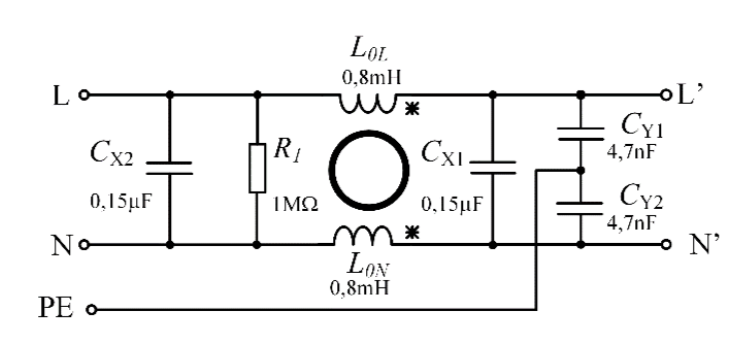
\includegraphics[width = 10cm]{orig_ElectricalCircuit.png}
	\caption{Original Schaltung \cite{aufgabenstellung}}
	\label{fig:orig_Schaltung}
\end{figure}

\bigskip